\documentclass[12pt]{article}

% Codificación y lenguaje
\usepackage[utf8]{inputenc}
\usepackage[spanish]{babel}

% Matemáticas
\usepackage{amsmath, amssymb}

% Tipografía y justificación
\usepackage{lmodern}
\usepackage{ragged2e} % Para justificar

% Tablas y figuras
\usepackage{graphicx}
\usepackage{caption}
\usepackage{float}
\usepackage{booktabs}
\usepackage{longtable}
\usepackage{array}
\usepackage{lscape}

% Diseño y formato
\usepackage[a4paper, margin=2.5cm]{geometry}
\usepackage{titlesec}
\usepackage{tcolorbox}

% Hipervínculos
\usepackage{hyperref}

% Para caracteres Unicode especiales
\DeclareUnicodeCharacter{202F}{\,}


\title{Materiales y Métodos}
\author{}
\date{}


\titleformat{\section}{\large\bfseries}{\thesection.}{0.5em}{}

\begin{document}

\begin{center}

%-----------------PARTE DE RONALDO-------------------------------
    \LARGE \textbf{Predictive Model for Inventory Management in Grocery Stores in Puno Using ARx and Integer Linear Programming}\\[0.5cm]
    
    \Large \textbf{Modelo predictivo para la gestión de inventarios en tiendas de abarrotes en Puno usando ARx y programación lineal entera}\\[0.5cm]
    
    \normalsize BUTRON MAQUERA TANIA KARIN\\
    CACERES TACORA ESTEFANY LIZBETH\\
    MAMANI MENA RONALDO CARLOS\\
    PAREDES COAGUILA FIORELLA YANETH\\
\end{center}

\vspace{0.5cm}

\begin{tcolorbox}[colback=gray!10, colframe=black, title=\normalsize Abstract]
\justifying
In the surroundings of the National University of the Altiplano, in the city of Puno, many small neighborhood stores face difficulties in estimating how much to buy to meet daily customer needs. During a visit to one of these stores, located two blocks from the local slaughterhouse, we collected real data provided by the shopkeeper, who kindly shared her experience, including how much she invests and how much she recovers. This study focuses on six frequently sold products: bread, chicken, rice, eggs, detergent, and shampoo. We used the ARx ARIMA model to forecast weekly demand and suggest optimal purchase quantities, aiming to avoid shortages or unnecessary surpluses. The goal is to demonstrate that time series models can help small businesses make better decisions and improve their earnings.

\textbf{Keywords}: optimization, ARx ARIMA, demand forecasting, groceries, inventory, time series.
\end{tcolorbox}

\vspace{0.5cm}

\section*{Resumen}
\justifying
En los alrededores de la Universidad Nacional del Altiplano, en la ciudad de Puno, muchas tiendas pequeñas tienen dificultades para calcular con precisión cuánto deben comprar para satisfacer la demanda diaria. Durante nuestra visita a una de estas tiendas, ubicada a dos cuadras del camal, la señora que atiende fue muy amable y nos compartió datos reales sobre su negocio, incluyendo cuánto invierte y cuánto logra recuperar en promedio. Este estudio toma como base seis productos que se venden constantemente: pan, pollo, arroz, huevo, detergente y shampoo. Aplicamos el modelo ARx ARIMA para predecir la demanda semanal de cada producto y así proponer una cantidad de compra más adecuada, evitando tanto el desabastecimiento como la sobrecompra. Con este trabajo, buscamos mostrar que el uso de modelos estadísticos puede ayudar mucho a los negocios pequeños a tomar mejores decisiones y manejar su inventario con más seguridad.

\textbf{Palabras clave}: optimización, ARx ARIMA, demanda, abarrotes, inventario, series temporales.

\vspace{0.5cm}

\section{Introducción}
\justifying
En la ciudad de Puno, muchas tiendas de abarrotes, especialmente las que se encuentran cerca de instituciones como la Universidad Nacional del Altiplano, atienden a una gran cantidad de personas cada semana. Estas tiendas, en su mayoría, funcionan gracias al esfuerzo diario de familias que trabajan con mucha dedicación, pero sin herramientas técnicas para planificar sus compras.

Durante una visita que realizamos a una tienda ubicada a dos cuadras del camal, pudimos conversar con la dueña, quien nos recibió con mucha amabilidad y nos brindó información clave sobre cómo maneja su negocio: cuánto invierte cada semana, qué productos son los que más se venden y cómo decide cuánto comprar.

A partir de esa experiencia, decidimos aplicar un modelo estadístico llamado ARx ARIMA para ayudar a predecir la demanda semanal de los productos más importantes en su tienda. Nos enfocamos en seis artículos básicos que casi todos los clientes buscan: pan, pollo, arroz, huevo, detergente y shampoo. Estos productos tienen una alta rotación y, si no se calculan bien las cantidades a comprar, pueden generar pérdidas por exceso o quedarse sin stock justo cuando más se necesitan.

Para el desarrollo del modelo, trabajamos con datos históricos de ventas semanales recopilados durante 72 semanas consecutivas. Sin embargo, el análisis se centró en estudiar de forma detallada las primeras 52 semanas —correspondientes a un año completo— con el objetivo de identificar patrones estacionales y comportamientos recurrentes. Estos patrones sirvieron de base para predecir la demanda en las semanas restantes, lo que permitió evaluar la precisión del modelo y su utilidad práctica en la planificación de compras.

Este trabajo tiene como objetivo encontrar la cantidad óptima que la tienda debería comprar cada semana, basada en los datos reales recogidos, para lograr una mejor organización de su inventario. Más allá del resultado numérico, queremos demostrar que incluso en negocios pequeños se puede aplicar la estadística y la programación para tomar decisiones más inteligentes y prácticas. Creemos que esta propuesta puede servir de ejemplo para otras tiendas de la ciudad, que enfrentan los mismos retos todos los días.



%----------------------------PARTE DE FIORELLA----------------------
\section{Materiales y Métodos}

\subsection{Base de Datos}

En este estudio, utilizamos un conjunto de datos sintéticos de ventas semanales de 6 productos de consumo diario en tiendas de vecindario, como se resume en la Tabla \ref{tabla:productos}. La elección se llevó a cabo al entrevistar a los vendedores en los distintos barrios de la ciudad de Puno; se escogieron estos productos porque reflejaban las ventas diarias durante el periodo de tiempo estudiado y exhiben un comportamiento constante a través del tiempo.

\begin{table}[H]
\centering
\caption{Productos seleccionados}
\label{tabla:productos}
\begin{tabular}{|c|l|}
\hline
Producto 1 & Pan        \\ \hline
Producto 2 & Pollo      \\ \hline
Producto 3 & Arroz      \\ \hline
Producto 4 & Huevo      \\ \hline
Producto 5 & Detergente \\ \hline
Producto 6 & Shampoo    \\ \hline
\end{tabular}
\end{table}
\vspace{0.5cm}
La demanda de cada producto por semana se muestrea durante un periodo de 78 semanas, es decir, los datos generados emulan la dinámica de las demandas por producto para este intervalo de ventas. Para evaluar la capacidad predictiva de los modelos, el dataset se segmenta en dos subconjuntos, como se puede observar en la Tabla \ref{tabla:segmentacion}.

\begin{table}[H]
\centering
\caption{Segmentación en subconjuntos}
\label{tabla:segmentacion}
\begin{tabular}{|l|c|c|}
\hline
Conjunto            & Semanas Incluidas & N° de Semanas \\ \hline
Entrenamiento       & 1 – 56            & 56            \\ \hline
Validación o prueba & 57 – 78           & 22            \\ \hline
\end{tabular}
\end{table}
\vspace{0.5cm}
Este particionamiento permite ajustar los modelos con 56 semanas de historial y luego medir su desempeño sobre 22 semanas “nuevas”, garantizando así una validación estricta fuera de muestra.

\vspace{0.5cm}

\textbf{Variables exógenas:} 
Para incorporar relaciones de influencia cruzada entre productos, en cada modelo de predicción, cada producto “objetivo” $i$ asumen las ventas de los otros cinco productos como variables exógenas que pueden influir en su demanda, de este modo, si el modelo predice la demanda de “pan”, las columnas de pollo, arroz, huevo, detergente y shampoo actúan como regresores externos (exógenos). De este modo, la matriz de variables explicativas en entrenamiento y prueba queda compuesta, para cada producto $i$, por las cinco series de ventas de los productos distintos de $i$, lo cual enriquece la fase de ajuste al captar posibles efectos de complementariedad o sustitución en la demanda semanal. 


\vspace{0.5cm}
\subsection{Modelado de la Demanda (ARIMAX)}

El modelo ARIMAX (AutoRegressive Integrated Moving Average with eXogenous variables) constituye una extensión de los modelos ARIMA clásicos, en los que se incorpora información adicional proveniente de variables externas que pueden tener influencia sobre la variable principal de estudio. En este caso, la demanda semanal de cada producto es modelada considerando tanto su comportamiento histórico como la posible interacción con las ventas de los otros productos. Esta estrategia permite capturar relaciones de complementariedad o sustitución entre bienes de consumo. Según Hyndman y Athanasopoulos (2018), los modelos ARIMAX son adecuados cuando se dispone de variables explicativas confiables que enriquecen la estructura predictiva del modelo.
\vspace{0.3cm}
Para modelar y predecir la demanda semanal de cada uno de los seis productos se emplea un enfoque de series de tiempo autorregresivas con regresores externos (ARIMAX). Se construyen y ajustan los modelos que permiten estimar la demanda semanal de cada uno de los seis productos a partir de sus propias ventas históricas y de las series de los demás productos como regresores externos. El objetivo es obtener para cada producto i una predicción que sirva luego de insumo al modelo de optimización. 
\vspace{0.3cm}
\begin{equation}
\hat{\mathbf{Y}}_i = \left\{ \hat{y}_{i,57}, \hat{y}_{i,58}, \ldots, \hat{y}_{i,78} \right\}
\end{equation}
Para cada producto definimos:
\begin{itemize}
    \item $\mathbf{Y}_i^{\text{entren}}$ son las ventas de la semana 1 a la 56.
\end{itemize}
\begin{itemize}
    \item $\mathbf{Y}_i^{\text{prueba}}$ son las ventas de la semana 57 a la 78.
\end{itemize}
\begin{itemize}
    \item $\mathbf{X}_i^{\text{entren}}$  y $\mathbf{X}_i^{\text{prueb}}$ son las matrices con los valores de las ventas de los productos en los mismos periodos.
\end{itemize}
\vspace{0.3cm}
La estrategia de ajuste y pronóstico se realiza en dos fases:

\begin{itemize}
    \item \textbf{Identificación y estimación del modelo:}

Utilizamos la función auto.arima() de la librería forecast en R, la cual selecciona automáticamente los órdenes minimizando el criterio de información AICc y determinando si es necesario diferenciar la serie para hacerla estacionaria.

Se especifica el argumento xreg = xreg\_entrenamiento, pasando la matriz de regresores externos formada por las ventas de los otros cinco productos durante las 56 semanas de entrenamiento.

    \item \textbf{Generación de pronósticos:}

Con el modelo estimado se invoca forecast (modelo\_i, xreg = xreg\_prueba, h = 22), obteniendo predicciones puntuales y sus intervalos de confianza para las semanas 57–78, que servirá como demanda esperada en la etapa de optimización entera.

En esta etapa xreg\_prueba contiene las ventas de las cinco variables exógenas en el período de validación.

\end{itemize}

\vspace{0.5cm}

De esta forma, cada modelo captura tanto la estructura temporal propia de la demanda de i (tendencia, estacionalidad o autocorrelación) como las posibles interdependencias con los demás productos, lo que suele mejorar la precisión frente a un ARX univariante clásico. El conjunto resultante de predicciones sirve de insumo para la siguiente fase de optimización entera de las cantidades a comprar.

\vspace{0.5cm}
\subsection{Entrenamiento y Validación del Modelo}

Con el objetivo de uniformizar las escalas entre productos, se evaluó la posibilidad de normalizar cada serie de tiempo. Sin embargo, dado que los modelos ARIMAX utilizados manejan adecuadamente las diferencias de magnitud y no se observaron mejoras sustanciales en los resultados, se trabajó directamente con los datos originales.
\vspace{0.3cm}
En esta etapa para cada producto objeto de estudio (pan, pollo, arroz, huevo, detergente y shampoo), se construye un modelo ARIMAX que combina la dinámica interna de la serie de ventas con el aporte de las cinco series restantes como regresores exógenos. El proceso de entrenamiento y validación se desarrolla a continuación:

\vspace{0.5cm}
\subsubsection{Ajuste de los Modelos ARIMAX}
En primer lugar, se extrae de la base de datos la porción correspondiente a las semanas 1 a 56 para cada producto i. Esta serie histórica entrena cada modelo usando \verb|auto.arima()| con los datos de entrenamiento y los regresores correspondientes minimizando el criterio de información AICc. Durante este ajuste, el algoritmo estima simultáneamente los coeficientes autorregresivos, de medias móviles y los parámetros asociados a cada uno de los cinco regresores exógenos (ventas de los demás productos), así como la varianza del término de error. Con ello, cada modelo captura tanto la autocorrelación propia de la demanda de i como la influencia que ejercen los productos complementarios o de sustitución.
\vspace{0.3cm}

Una vez ajustado el modelo para cada producto, se evalúa su capacidad predictiva sobre el conjunto de validación, formado por las semanas 57 a 78. Para ello, se generan pronósticos puntuales de demanda usando las ventas de los regresores en ese periodo.  
\vspace{0.3cm}
\begin{equation}
\hat{y}_{i,57:78} = \text{forecast}(modelo_i, \ xreg = \mathbf{X}_i^{\text{prueba}}, \ h = 22)
\end{equation}

donde $\mathbf{X}_-i^{\text{prueba}}$ es la matriz de regresores exógenos real de las semanas de validación.

\vspace{0.5cm}
\subsubsection{Métricas de Desempeño}

Para evaluar la precisión de los modelos de predicción, se utilizan métricas estadísticas comúnmente aplicadas en el análisis de series temporales. Estas permiten cuantificar la diferencia entre los valores reales y los valores estimados, tanto en términos absolutos como relativos. 

\begin{itemize}
    \item \textbf{MAE \textbf{(Mean Absolute Error / Error Absoluto Medio)} 
}Esta métrica calcula el promedio de las diferencias absolutas entre los valores reales y los valores pronosticados. Es una medida directa del error promedio sin considerar su dirección. Un valor bajo de MAE indica que el modelo tiene una buena capacidad de aproximación a los datos.
\textbf{
    \begin{equation}
        \text{MAE} = \frac{1}{n} \sum_{t=1}^{n} | y_t - \hat{y}_t |
    \end{equation}
    \item \textbf{RMSE (Root Mean Squared Error / Raíz del Error Cuadrático Medio)} }
Esta métrica penaliza con mayor severidad los errores grandes, ya que eleva al cuadrado las diferencias antes de promediarlas. Es útil para detectar modelos que pueden tener errores extremos. Un RMSE bajo refleja una alta precisión en la predicción.

    \begin{equation}
        \text{RMSE} = \sqrt{\frac{1}{n} \sum_{t=1}^{n} ( y_t - \hat{y}_t )^2}
    \end{equation}
    \item \textbf{MAPE (Mean Absolute Percentage Error / Error Porcentual Absoluto Medio }
Esta métrica expresa el error en forma porcentual con respecto a los valores reales, permitiendo comparar el desempeño entre series con diferentes magnitudes. Es particularmente útil cuando se desea interpretar la precisión en términos relativos. Sin embargo, puede volverse inestable cuando los valores reales tienden a cero. 
    \begin{equation}
        \text{MAPE} = \frac{100}{n} \sum_{t=1}^{n} \left| \frac{y_t - \hat{y}_t}{y_t} \right|
    \end{equation}
\end{itemize}

Los resultados de estas métricas para cada producto permiten identificar cuál modelo presenta el mejor desempeño en términos de exactitud y robustez. Estas predicciones constituyen la base para la siguiente fase de optimización de decisiones de compra.

\vspace{0.5cm}
\subsection{Programación Lineal Entera}

La programación lineal entera (ILP, por sus siglas en inglés) es una técnica de optimización utilizada para resolver problemas en los que las variables de decisión toman únicamente valores enteros. Su aplicación es especialmente útil en contextos de decisiones discretas, como la planificación de compras con presupuestos limitados. En el presente estudio, la ILP se utiliza para maximizar la utilidad esperada de las compras semanales, considerando las predicciones de demanda como límites superiores de adquisición y las restricciones impuestas por el presupuesto del comerciante. Tal como lo indican Winston y Goldberg (2004), este tipo de modelos resulta adecuado para representar problemas logísticos y financieros en escenarios reales.

%----------------------------PARTE DE TANIA-----------------------
\section{Resultados}

La presente sección expone los principales hallazgos derivados del análisis de series temporales multivariadas y de la implementación de un modelo de optimización basado en programación lineal entera. El objetivo fue predecir la demanda semanal de seis productos esenciales y, con base en dichas predicciones, maximizar la rentabilidad de las compras respetando una restricción presupuestaria semanal.

\subsection{Predicción de la demanda}

Posterior a la aplicacion del modelo ARX (AutoRegresivo con variables exógenas) para predecir la demanda de los productos: pan, pollo, arroz, huevo, detergente y shampoo. Las predicciones se realizaron sobre un horizonte de 22 semanas, utilizando los datos históricos de ventas correspondientes a las primeras 56 semanas como conjunto de entrenamiento. Las variables exógenas utilizadas fueron las ventas de los otros productos, bajo el supuesto de que podrían influir entre sí.

Para evaluar el desempeño del modelo en cada producto, se calcularon las métricas MAE (Error Absoluto Medio), RMSE (Raíz del Error Cuadrático Medio) y MAPE (Error Porcentual Absoluto Medio). Estas métricas indicaron niveles aceptables de precisión en la mayoría de los casos, lo cual respalda la viabilidad del modelo para estimar la demanda futura.
\begin{figure}[H]
    \centering
    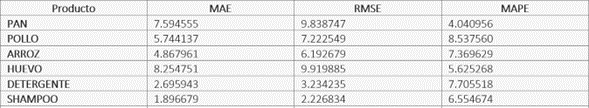
\includegraphics[width=0.8\textwidth]{error.png}
    \caption{MAE(Error Absoluto Medio), RMSE (Ráız del Error Cuadrático Medio) y MAPE (Error Porcentual Absoluto Medio)}
\end{figure}
Las visualizaciones correspondientes a cada producto mostraron una concordancia adecuada entre las series reales y las series predichas, lo que sugiere que el modelo logra capturar adecuadamente la tendencia y la estacionalidad de las ventas. En productos como el arroz y el pollo, la precisión fue mayor, mientras que en productos como el shampoo, las predicciones presentaron una mayor variabilidad.



\begin{figure}[H]
    \centering
    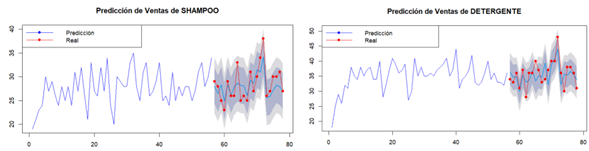
\includegraphics[width=0.8\textwidth]{Ima11.png}
    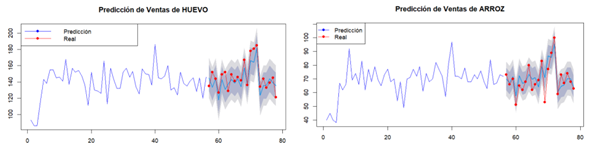
\includegraphics[width=0.8\textwidth]{Ima22.png}
    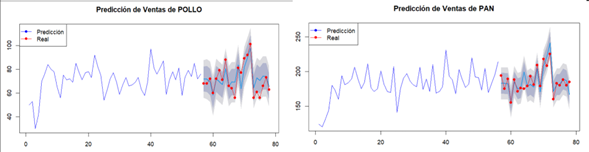
\includegraphics[width=0.8\textwidth]{Ima33.png}
    \caption{Predicción vs. datos reales para cada uno de los productos}
\end{figure}

\subsection{Optimización de decisiones de compra}

Posteriormente, se procedió a optimizar las decisiones de compra semanales mediante la formulación de un problema de programación lineal entera (ILP). El objetivo de la optimización fue maximizar la ganancia semanal, definida como la diferencia entre el ingreso por ventas (precio de venta por unidad) y el costo de adquisición de cada producto.

Para cada semana, se impusieron dos restricciones:
\begin{itemize}
    \item Un límite presupuestario máximo de S/. 500.
    \item No exceder la cantidad predicha como demanda semanal.
\end{itemize}

Los resultados obtenidos evidencian una asignación eficiente del presupuesto semanal, priorizando productos con mayor rentabilidad relativa. El modelo permitió identificar, semana a semana, la combinación óptima de unidades a adquirir para cada producto, asegurando una utilización racional del presupuesto y un retorno económico favorable.


\begin{figure}[H]
    \centering
    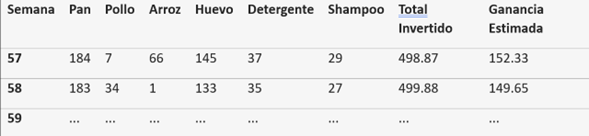
\includegraphics[width=0.75\textwidth]{tablaPRED.png}
    \caption{Resumen de compras óptimas y ganancias semanales (semanas 57–78)}
\end{figure}

\subsection{Análisis visual de los resultados}

Se elaboraron visualizaciones que permiten observar de manera clara la evolución de los indicadores clave:

\textbf{Inversión y ganancia semanal (semanas 57–78):} La inversión se mantuvo cerca del límite presupuestal en la mayoría de las semanas, lo cual refleja un aprovechamiento casi completo del presupuesto disponible. En cuanto a la ganancia, esta se situó en un rango relativamente estable, con valores superiores a los S/. 150 por semana, alcanzando picos cercanos a S/. 190, dependiendo de la demanda proyectada y los márgenes de ganancia de los productos priorizados.

\begin{figure}[H]
    \centering
    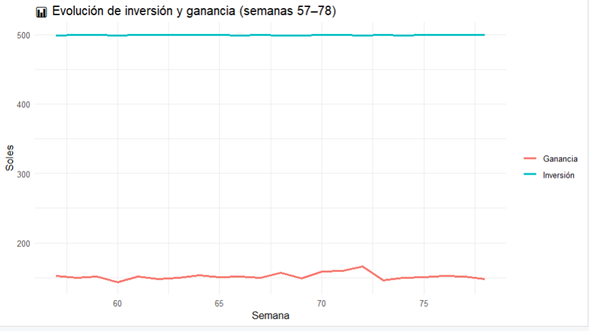
\includegraphics[width=0.75\textwidth]{Imagen3.png}
    \caption{Evolución de la inversión y ganancia semanal (semanas 57–78)}
\end{figure}

\textbf{Unidades adquiridas por producto:} El análisis gráfico de las cantidades compradas por semana mostró comportamientos diferenciados por producto. El pollo y el arroz, por su alto margen de ganancia y demanda estable, fueron adquiridos de forma constante. En contraste, productos como el shampoo y el detergente mostraron compras más intermitentes, influenciadas tanto por su demanda proyectada como por su menor rentabilidad relativa.

\begin{figure}[H]
    \centering
    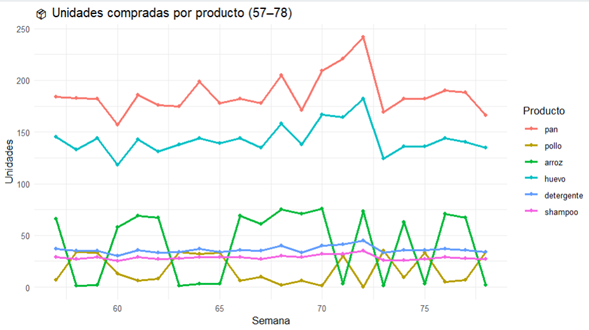
\includegraphics[width=0.8\textwidth]{uproducto1.png}
    \caption{Evolución semanal de unidades adquiridas por producto}
\end{figure}

Estos resultados reflejan el éxito del enfoque adoptado al integrar técnicas de predicción con métodos de optimización, proporcionando una herramienta efectiva para la toma de decisiones en contextos de planificación de inventarios bajo restricciones financieras.




%MI PARTE 
\section{Discución y Conclusión}
Los hallazgos derivados del presente estudio demuestran la efectividad de una estrategia integrada que combina modelos de predicción basados en series temporales multivariadas con técnicas de optimización matemática para la toma de decisiones en la gestión de compras. En particular, la aplicación del modelo autorregresivo con variables exógenas (ARX) permitió estimar con un nivel aceptable de precisión la demanda futura de seis productos esenciales, destacándose un mejor desempeño en aquellos con patrones de consumo más regulares (p. ej., arroz y pollo), en comparación con productos de comportamiento más errático, como el shampoo.
\vspace{0.4cm}
Las métricas de evaluación (MAE, RMSE y MAPE) reflejaron niveles de error dentro de rangos operativamente tolerables, lo cual valida el uso del modelo ARX como herramienta predictiva en entornos reales. Cabe destacar que la incorporación de variables exógenas resultó relevante para capturar interrelaciones entre productos, contribuyendo a una mayor robustez en las proyecciones.
\vspace{0.4cm}
En la segunda etapa, la formulación de un modelo de programación lineal entera (ILP) facilitó la toma de decisiones óptimas de compra, maximizando la utilidad semanal bajo restricciones de presupuesto e inventario proyectado. El modelo mostró un uso eficiente de los recursos disponibles, alcanzando niveles de inversión cercanos al umbral máximo permitido (S/. 500) y generando ganancias semanales estables superiores a S/. 150. Esta asignación racional se reflejó en la priorización de productos con alta rentabilidad relativa, tal como evidencian los resultados gráficos y tabulares.
\vspace{0.4cm}
Desde una perspectiva aplicada, la integración entre modelos predictivos y optimización matemática representa una herramienta poderosa para la planificación táctica de inventarios en entornos de alta variabilidad y recursos limitados. Los resultados respaldan la utilidad del enfoque propuesto para mejorar la eficiencia operativa y económica en contextos similares.
\vspace{0.4cm}
Como proyección futura, se recomienda explorar modelos estocásticos que incorporen incertidumbre explícita en la demanda, así como considerar dinámicas adicionales como variaciones en precios, costos logísticos o penalizaciones por desabastecimiento. Estas extensiones podrían contribuir a una representación más realista y a una toma de decisiones aún más robusta.

\section{Referencia }
\begin{itemize}
    \item Box, G. E. P., Jenkins, G. M., Reinsel, G. C., \& Ljung, G. M. (2015). \textit{Time Series Analysis: Forecasting and Control} (5th ed.). Wiley.
    \item Hyndman, R. J., \& Athanasopoulos, G. (2018). \textit{Forecasting: Principles and Practice} (2nd ed.). OTexts. \url{https://otexts.com/fpp2/}
    \item Henao-Baena, C. A., Zuluaga-Zuluaga, B., Galeano-Castro, J., Marin-Garcia, E. J., \& Calvo-Salcedo, A. F. (2024). \textit{Methodology for inventory management in neighborhood stores using machine learning and integer linear programming.} Ingeniería, 29(1), 206–221. \url{https://doi.org/10.14483/23448393.19423}
    \item Winston, W. L. (2004). \textit{Operations Research: Applications and Algorithms} (4th ed.). Duxbury Press.
    \item Laporte, G. (1992). The vehicle routing problem: An overview of exact and approximate algorithms. \textit{European Journal of Operational Research, 59}(3), 345–358.
    \item Makridakis, S., Wheelwright, S. C., \& Hyndman, R. J. (1998). \textit{Forecasting: Methods and Applications} (3rd ed.). Wiley.
\end{itemize}

\section{Anexos}
\subsection{Anexo 1: Visita a al tienda de barrio:}
\begin{figure}[H]
    \centering
    
\includegraphics[width=0.7\textwidth]{grupo.jpg}
    \caption{Fotografía del grupo entrevistando a la dueña de una tienda local como parte de una actividad de recolección de información.}
\end{figure}
\subsection{Resgitro de boletas de negocio}
\begin{figure}[H]
    \centering
    \includegraphics[width=0.5\textwidth]{boletas.png}
    \caption{La fotografía muestra los grupos de boletas que la dueña de la tienda presentó como parte de su documentación comercial.}
\end{figure}

\end{document}
